\chapter{Discussion}
\label{chap:discussion}

% THE ENTIRE AND SOLE POINT OF THE DISCUSSION SECTION SHOULD BE TO INTERPRET
% THE RESULTS AS TO WHETHER THE CIDR REPORT EVER WAS EFFECTIVE AND THEN, BASED
% ON THE OBSERVED CHANGES, WHETHER IT BECAME LESS EFFECTIVE OR WHETHER
% SOMETHING ELSE CAUSED THE OBSERVED BEHAVIORAL CHANGE
%
% \fbox{Look at Tony Li's interview again}

The figures and analysis presented thus far have provided some insight about
the behavior of ASes appearing on the CIDR Report and general characteristics
about the CIDR Report itself. However, the process of re-implementing the
aggregation report and analyzing and observing AS behavior changes has also
raised a number of broader and more qualitative questions about the report
that we address in this chapter. We first discuss whether the CIDR Report was
accurate and whether it was effective using broader definitions of these terms
than were used in the analysis proper, and then discuss potential hypotheses
for why the response to appearing on the CIDR Report changed over time, both as
observed during the analysis and as claimed qualitatively by network operators.
Finally, we consider the CIDR Report and Internet routing table CPR in the
context of Ostrom's design principles for CPR governance institutions.

\section{Is the CIDR Report accurate?}
While part of the first section of the previous chapter was dedicated to the
question of whether our implementation of the aggregation report produced
similar output to that of the authoritative CIDR Report, we did not address the
larger questions of whether the CIDR Report is representative of the problems
observed by operators regarding deaggregation and routing table growth. These
issues are important to the CIDR Report's efficacy and trustworthiness as a
monitoring tool in support of the social forces influencing Internet routing
and aggregation, and yet are not definitively addressed; there is simply a lack
of obvious complaints or criticisms from network operators in public channels.

\paragraph{Is the CIDR Report's vantage point representative?}
The first observation we make is with regard to representativeness of the
routing table and aggregation potential observed and presented on the CIDR
Report as compared to what other network operators observe in their own routing
tables. The nature of BGP and policy-controlled route selection and propagation
make it possible for two networks to have different views and different numbers
of prefixes in their ``full'' routing table, due to the routing policies of the
networks they interconnect with. Ostensibly if the CIDR Report reports behavior
that does not represent what most other networks observe, the CIDR Report will
be less credible and more likely to be disregarded by network operators.
Unfortunately it is difficult to characterize what a representative routing
table might contain precisely because of this nature of BGP.

It would seem that the default-free zone (DFZ), the routing table maintained by
the major default-free providers that form the root of our roughly-hierarchical
Internet, is a reasonable place to take this measurement from. DFZ network
operators must theoretically maintain the fullest routing tables in order to
achieve full Internet reachability, and versions of these routing tables are
shared with DFZ customers. In cases of interactions between large
non-DFZ networks, such as major content provider or ``eyeball'' networks,
routes may be observed that are not globally visible, but it is reasonable to
expect problems related to excessive routes advertised between peers to be
resolved via normal peering dispute resolution approaches.

Reasonable proxies for the DFZ have been used as vantage points for the
authoritative CIDR Report since its inception, as identified in
Table \ref{table:cr_vantage_points}, as well as the analysis in this thesis.
However, the DFZ routing table may still not be completely representative.
Large providers receive routes from many peers and other providers, and so must
maintain a RIB that is several multiples larger than the DFZ operational
routing table or FIB, which is composed of only the best routes from the RIB.
Further, the route export policies of ISPs adjacent to the vantage point for
the CIDR Report may also affect the degree to which the CIDR Report represents
most providers routing tables. For example, in our analysis using Route Views
as a vantage point, there were cases where the DFZ and other large providers
all reported similar numbers of prefixes, while a smaller Route Views peer
reported an order of magnitude more. These additional prefixes appeared to be
in support of traffic engineering, and the AS that was ``leaking'' these
prefixes into Route Views was likely not respecting a NO-EXPORT policy that had
been applied to these routes from their origin AS\footnote{This problem was
confirmed to affect the authoritative CIDR Report as well, through indirect
correspondence with Patrick Gilmore.}. Thus, without knowing the configuration
of the export policy of peers and other providers that contribute a large
fraction of the routes to the BGP view of the vantage point, it is possible
that a non-representative view of the routing table may be generated, leading
to a non-representative CIDR Report.

% -best path only -- potentially blocks aggregation
% -filtering vs. everything for an anlytics perspective
%      Route export policy for customers vs. for CIDR Report -- i.e. routeviews
%     - no-export and other communities
%     -consensus vs. a single source vs. something in between
%
% \begin{quote}
% P.S. The list is not 100\% correct.  For instance, tw telecom has
% no-export set on their de-agg prefixes.  This means those de-aggs don't hit the
% global table, just their transit provider.  But if Geoff peers with the transit
% provider directly, he may see them (even though he should not).  I have spoken
% to tw telecom about this face-to-face.  (Part of that "shaming" thing.)
% \end{quote}

\paragraph{Is all deaggregation equally problematic?}
All route announcements that consume slots in the routing table incur the same
cost in that they consume a fraction of the router's resources that cannot be
utilized by another route. However, as the Internet has changed in purpose and
structure over time, the need to perform certain tasks (multihoming, TE) in BGP
that result in route deaggregation and increased numbers of prefixes in the
routing table have been motivated by network management and engineering. The
norms of the Internet operations community appear to have recalibrated
accordingly, seemingly assigning different value to the benefit and
justifiability of different deaggregation-inducing behavior.

While there are different views on the subject \cite{Li:2011vn}, most seem to
conclude that route announcements due to multihoming and prefix hijacking
prevention are unavoidable and justifiable, while traffic engineering is less
so, especially in the case of fine-grained TE by large residential access ISPs
\cite{Steenbergen:2010nx}. Worst of all is the failure to aggregate or
announcement of ``class C'' blocks in the era of CIDR. Such behavior indicates
a lack of ``clue'' and provides no benefit to anyone, and so is universally
deplored.

Distinguishing between these behaviors is often difficult, as the information
required to discern the intent of deaggregation is not always available from
the vantage point routing tables accessible for measurements. \cite{Bu:2004fk}
present a definition for measuring multihoming and \cite{Cittadini:2010pi}
present some measurement techniques for observing traffic engineering. However,
other forms of traffic engineering between large ASes may not be visible
because it is based on routing parameters such as NEXT\_HOP that are not
visible from adjacent ASes \cite{Steenbergen:2010nx}.

Regardless of the measurability of these various phenomena, the CIDR Report
does not attempt to measure or distinguish between any of the causes or
underlying intentions of deaggregation, instead simply reporting the number of
prefixes announced by each AS that appear aggregable from the CIDR Report's
vantage point. While this is a true representation of each AS' contributions to
the routing table, it does not accurately reflect the relative values
attributed to aggregation by network operators. Thus, some operators may
conclude that the report is not as useful because it does not distinguish
between these behaviors. Further, because some of these
purposefully-deaggregated routes are difficult to withdraw, they may lead to
some ASes appearing in unmoving positions on the CIDR Report, as hypothesized
in \cite{Steenbergen:2010nx}.

\section{Is the CIDR Report effective?}
While the section of the previous chapter analyzing the post-treatment behavior
of ASes appearing on the CIDR Report addressed the question of whether the CIDR
Report appeared to correlate with AS behavior change, it did not address the
more general question of the CIDR Report's purpose and use by operators:
initially to encourage aggregation following the adoption of CIDR and BGP-4,
and then later and more generally to encourage efficient route announcements by
providing monitoring information about the greatest deviation from community
norms.

While the validity concerns identified previously limit our ability to draw
strong, causal conclusions, it does appear that the CIDR report had some effect
on the aggregation behavior of individual ASes, especially early on in the
study period. Further, in the very early days of CIDR, there is evidence of the
total number of prefixes in the routing table actually decreasing over time as
aggregation occurred. However, during the period studied in this thesis, the
routing table generally grows continuously over time, as was shown in Figure
\ref{fig:huston_table_plot}.

\paragraph{Considering the counterfactual (no CIDR Report) world}
The ideal measure of general CIDR Report efficacy would be to observe route
announcement and aggregation behavior in the counterfactual world where the
CIDR Report does not exist. While we cannot actually observe this, we can
construct an estimate of the counterfactual routing table under the assumption
that without a CIDR Report, networks might not withdraw announcements, instead
leaving them in the routing table. By observing the cumulative number of
prefixes advertised for at least some period of time, we could construct an
upper bound of the counterfactual routing table size. A plot of these
counterfactual routing table sizes is shown in Figure \ref{fig:counterfactual}.

\begin{figure}[h]
\begin{center}
    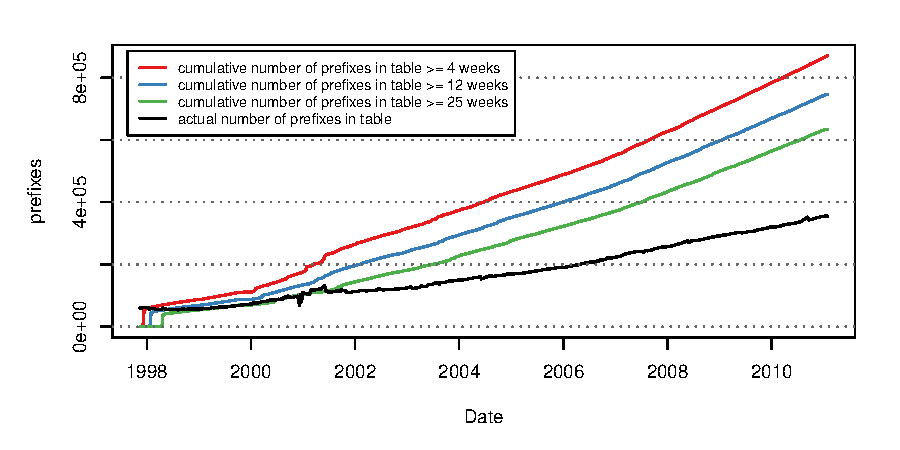
\includegraphics[width=6in]{figures/counterfactual.pdf}
    \vspace{-2em}\\
    \caption{Counterfactual routing table prefix counts over time.}
    \label{fig:counterfactual}
\end{center}
\end{figure}

As illustrated in this figure, the number of prefixes in the counterfactual
table size grows faster and eventually larger than the actual routing table
size, even for conservative estimates of how many weeks a prefix must be in the
routing table for it to constitute a ``permanent'' prefix. While the
construction of this counterfactual is far from methodologically perfect, it
provides further evidence that the CIDR Report or some other aspect of the
network operations community had some effect on route aggregation behavior. The
deviation between this counterfactual plot and the actual size of the routing
table could alternately be interpreted as evidence that there is a tendency
for aggregation or route withdrawal to occur naturally without appearing (or
fear of appearing) by the CIDR Report, though this is disputed by the behavior
of the control group in the previous chapter.

% In spite of seeing aggregation behavior relative to the control, the total
% number of routes in the routing table does not drop over time, suggesting that
% old people are replaced by new ``bad guys'' or new entrants. Cittadini's study
% suggests that the proportion of ``bad guys'' remains the same over time (the
% people that would show up on the CIDR Report), suggesting the rolling-over bad
% guy theory.
%
% OR. The table just grew less quickly than it otherwise could have, but we can't
% examine the counterfactual world...?
%
% Rolling-over bad guy theory would be supported by the rate of growth of new
% ASes on teh CIDR Report?
%
% Arthur suggests looking at the fraction (\# of /24s / \# of prefixes in the
% routing table) per AS or for the entire routing table, over time
%
% What do Cittadini's observations mean for my analysis of the later repport
% where people are far more deaggregated

\paragraph{How quickly should the CIDR Report take effect?}

This is a minor observation, but there is a question that arises from observing
the metrics selected for measurement in the previous chapter over time, such as
in Figure \ref{fig:delta_rel_netgain_cdf}. From this and other figures
presented over the various measurement periods from 30-730 days after the
initial appearance on the CIDR Report, we can see that some improvement (and
more generally change) occurs after 30 days, and often continues up to 730 days
after, though most of the observed change appears to occur between 30 and 365
days rather than than 365 and 730 days (one and two years). It seems reasonable
to assume that because most of the net change was observed to take place in the
first year after the initial CIDR Report appearance, it was likely related to
appearing on the CIDR Report and not some other phenomenon such as regression
to the mean. However, this argument is somewhat speculative in that we do not
understand the underlying mechanisms that cause the behavior changes observed.

% As those that have been treated by the CIDR Report have become more outliers
% over time, it's possible that those below the outliers may have been more
% susceptible to treatmetn. Or, they may have moved on tehir own -- it would be
% interesting to sample those with netgain comparable to 1998 CIDR report from
% 2011 and see if the behavior is more similar to 1998 or 2011.

\section{What caused the decrease in treatment effect over time?}
If we agree that there was a behavior change by ASes in response to appearing
on the report, then as we see the diminishing difference in behavior change
over time in the previous chapter, we conclude that the governance system
influenced by the CIDR Report became less effective over time. This agrees with
operator observations about the decline of the CIDR Report. However, these
observations do not offer any insight about what may have occurred within the
interdomain routing system and the Internet operations community surrounding it
to cause these changes.

Ostrom's model of rational appropriators, introduced in Chapter
\ref{chap:intro}, sets out four factors that influence the behaviors and
decision-making of appropriators. These are:
\begin{itemize}
    \item{internal discount rate: the relative perceived value of future
    benefits versus present benefits}
    \item{internal norms: internal values that influence the selection and
    relative valuation of strategies (which may in part be the result of
    externalizing internal norms)}
    \item{external costs: costs incurred from a particular strategy}
    \item{external benefits: benefits gained from a particular strategy}
\end{itemize}
By considering external changes and events over the course of the study period
that may have influenced these factors, we may be able to develop hypotheses
for the observed behavior change. While we cannot conclusively attribute the
observed behavior change to any or all of these hypotheses, they are certainly
potential causes that could be investigated further in future.

In Ostrom's work, the discount rate is typically used to describe the ease by
which an appropriator may make their livelihood from another resource system,
thus freeing them from considering the future consequences of opportunistic
behavior in the current resource system.  In the case of the routing table and
the Internet more generally, there is only one, and so we will not consider the
internal discount rate, instead focusing on the other three factors in turn
below.

\paragraph{Changing community norms and responses}
While the criterion that Ostrom identifies here is internal norms, it could be
argued that most of the internal norms of participants in the Internet
community are motivated by the collective norms of the community. We thus focus
on these specifically.

In its very early days, the Internet operations and engineering community was
relatively small and homogeneous. Consisting of groups such as the IETF or the
NSFNET Regional Techs group (the forerunner of NANOG), these groups were
relatively small, met in-person frequently, and otherwise kept in close contact
via email mailing lists. These groups were composed of relatively consistent
participants that were mostly American and affiliated with equipment vendors,
service providers, contractors, and organizations that operated
Internet-connected networks---academic and educational institutions.
Individuals and their organizations had reputations to maintain in the Internet
meritocracy, and without motivation by commercial and competitive forces, this
community was more focused on collective welfare than on individual benefit
\cite{Li:2011vn}.

As the Internet has grown over time, the operations and engineering community
surrounding and supporting it has also grown and changed. First, as the
Internet has grown in importance and deployment outside of the United States,
the community of operators that participate in BGP operations has grown to
include a much more diverse group of people that no longer meet together or
participate on the same mailing lists, or who even speak the same language or
hold the same cultural norms and values. While there are still strong and
vibrant operator communities such as NANOG, RIPE, etc. these are all generally
regional rather than global. Further, and perhaps more important is that with
the transition of Internet service provision to a highly competitive commercial
activity, considerations of the benefit or cost of a particular activity to the
community are no longer considered, or at best considered after
profit-maximizing activities \cite{Li:2011vn}. Under such a mindset, reducing
ones impact on the routing table would at best be not in support of an ISP's
core business and at worst could be viewed to harm their Internet operations,
and so aggregation has become less of a concern to large, modern ISPs.

% - community has grown and become less homogeneous
%     - originally IETF + Regional-Tech, etc. with a common ethos, frequent
%       meetings (Tony Li)
%     - now all over the world (harder to communicate), commmerically motivated
%         - still pockets of this -- NANOG, etc.
%         - the inner circle of operators is still probably strong and pwerful
%     - clue doesn't matter anymore -- no longer a pride issue.

Finally, the attitude that the CIDR Report had become ineffective, espoused by
many of the operators that we spoke with, may have also played a role in the
change in effectiveness of the CIDR Report. Given that it only provides
information, the CIDR Report may only help improve aggregation of the routing
table through social action in the Internet operations community. If leading
operators deemed the report to have become ineffective, then there would be
little reason for them to continue to apply pressure via social forces, as it
would be a waste of time, or others would free-ride off of their efforts. Thus,
if this attitude was pervasive, it may have been a self-fulfilling prophecy
that changed attitudes and responses to the CIDR Report.

% source of ossification?

\paragraph{Changing benefits of routing deaggregation}
As discussed earlier, there are now greater engineering motivations to utilize
deaggregation to achieve reliability or performance goals via multihoming,
traffic engineering, and separate announcement of critical infrastructure
addresses to avoid route hijacking. While there are questions about the degree
to which this behavior has changed over time \cite{Cittadini:2010pi}, these
behaviors are certainly considered a normal part of BGP network operation now
whereas there were arguably less critical and more unusual in the era of a more
hierarchical Internet \cite{Labovitz:2010zr}.

Perversely, it has also been claimed (but not substantiated) that appearing on
the CIDR Report has been viewed by some as a positive indication for marketing
purposes \cite{Smith:2006vn}, presumably because it suggested that one operated
a large network like others appearing on the CIDR Report.

\paragraph{Changing costs of routing deaggregation}
The costs of routing deaggregation also appear to have changed over time, both
in terms of the marginal cost of a slot in a modern router and in terms of the
community response to operating a highly deaggregated network. First, in terms
of the marginal cost of a route, typical modern routers now have capacity for
several million routing table entries. This demand for routing table slots has
apparently been driven by the popularity of BGP/MPLS VPNs \cite{rfc2547} and the
business models they enable for ISPs, leading to the present where major
customers of a prolific router vendor do not seem to express concerns about the
Internet routing table's contributions to the total demand for routing table
slots \cite{Davie:2011uq}. This has made each routing table slot less valuable
over time. While aggregable prefixes still consume a significant fraction
of the total prefixes in the Internet routing table, the benefit of taking
action to encourage others to aggregate their routes has likely decreased over
time as slots have become less scarce.

In addition to the decreased cost of routing table slots, it appears that the
community response to announcing aggregable routes has decreased over time,
making it less costly in terms of reputation and criticism to announce
deaggregated prefixes. It is not possible to observe a measure of all
criticism in response to the CIDR Report, but we can consider a reasonable
proxy---the public discussion of the CIDR Report on the NANOG mailing list. A
figure of the frequency of mail messages containing ``CIDR R'' in the subject
line over the study period is shown below in Figure \ref{fig:mail-freq}.

\begin{figure}[h]
\begin{center}
    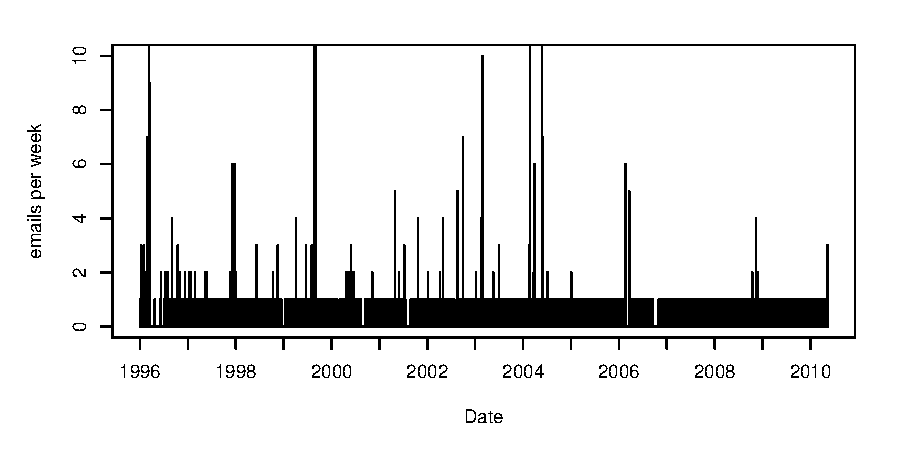
\includegraphics[width=6in]{figures/cr_email_freq.pdf}
    \vspace{-2em}\\
    \caption{Incidence of email messages containing ``CIDR R'' in the subject
    line, transmitted to the NANOG mailing list over 1996-2011.}
    \label{fig:mail-freq}
\end{center}
\end{figure}

This figure illustrates that while email discussion of the weekly CIDR Report
was fairly vigorous (including both commendations for improvement and criticism
for getting worse), these comments and conversations have essentially stopped
completely as of late. While this is probably coupled to the changes in
community norms discussed above, it also suggests that the criticism and thus
reputational ``cost'' of appearing on the CIDR Report has decreased over time.

\section{Learning from the CIDR Report and the routing table CPR system}

In spite of our discussion of governance institutions and Ostrom's CPR
framework at a number of points throughout this thesis, it is important to note
that the CIDR Report itself is not a CPR governance institution as Ostrom's
framework defines them. As noted in the introduction, such institutions require
participants to agree to make commitments to certain behavior, and typically
offer graduated sanctions to prevent opportunism in the event that monitoring
activities show deviation from commitment. In this context, the CIDR Report
fills a monitoring role that feeds into the loosely defined governance
customs that have been developed by network operators participating in the
Internet.

Ostrom \cite{Ostrom:1990fv} identifies five design principles\footnote{
The five identified for credible commitment are: clearly defined boundaries,
congruence between CPR rules and conditions, collective choice arrangements,
monitoring, and graduated sanctions. Ostrom also identifies three other
principles that, when absent, have caused failures in other CPR governance
institutions: dispute resolution mechanisms, recognition and non-interference of
the right to organize, and the use of nested enterprises in large-scale
systems}
necessary for participants in a CPR to make credible commitments to
follow agreed-upon rules. We discuss principles particularly relevant to the
CIDR Report and routing table governance institution below, while only touching
on principles that are less relevant or already satisfied.

% learning from the CIDR Report
% - not actually a governance institution -- just something some people created
%       -- maybe part of one, but AFAWK, it is completely norm-based -- there was
%       no collective action to supply an institution in the first place

\paragraph{Collective choice}
Perhaps the biggest challenge facing both the CIDR Report and the community
norm-based approach as a method of managing routing table growth is that none
of these mechanisms or the rules or principles that underlie them were ever
explicitly agreed upon or developed through a process by participants in the
interdomain routing system. Thus, when the community shared a collective set
of norms and principles regarding maintaining reputation, minimizing
deaggregation, etc., the CIDR Report provided a monitoring service according to
these norms and identified ASes that deviated from them most significantly.
With this information, community members who shared these norms could then
apply social pressure or assist the deviating ASes in improving their
aggregation behavior.

However, as these norms changed and the community also changed, there was no
precedent or process by which to achieve collective action to adjust the rules
to meet these changes and the interests of network operators accordingly. Thus,
the CIDR Report could not necessarily evolve to meet the interests of all, and
there was no obvious venue for network operators to participate in order to
change the CIDR Report or the rules and expectations of the community. Ostrom
would suggest that these reasons lessen the incentive for individuals to commit
to the rules of the routing table CPR, and ostensibly also played a role in the
apparent reduced efficacy and relevance of the report over time.

\paragraph{Monitoring}
The design principle most relevant to the CIDR Report is that of monitoring, as
it is the primary role of the CIDR Report. Monitoring, along with sanctions,
are essential to maintaining cooperation and limiting opportunistic behavior in
the long-running CPR institutions that Ostrom observes opportunistic behavior,
even in communities with shared norms and interest in reputation maintenance.
Internal monitoring and sanctioning provide assurances to participants making
commitments to abide by the rules that their trust will not be taken advantage
of---that opportunists will be detected and punished.

In consideration of Ostrom's principles, the CIDR Report is a reasonable
monitoring mechanism: it is provided by and can be verified by participants,
and is of low cost relative to sanction mechanisms. However, it is not ideal,
especially as it has remained static while the Internet has evolved.  In
addition to the specific issues of vantage points, accuracy, and interpretation
mentioned earlier, the CIDR Report only identifies the thirty most extreme
deaggregators in the network each week. While a limit on the number of networks
identified each week is arguably necessary because the social response to the
CIDR Report is a necessarily a human process that can only cope with a limited
amount of information, it has not scaled as the Internet has grown. Instead, as
illustrated in Figures \ref{fig:netcompare} and \ref{fig:netgain_cdf}, it now
focuses on significantly deaggregated outliers---0.1\% of the routing system
participants with 20\% of the prefixes.

This group of outliers may indeed be deserving of community attention, but the
limit of 30 ASes also ignores the next 20\% of the population that is
collectively responsible for the remaining 80\% of the aggregable prefixes.
These participants may be significantly deaggregated in relative terms and may
be in positions to easily improve their aggregation behavior but, because of
their relative size, never appear above the threshold of thirty. With the
current and historic trend of a constantly increasing minimum threshold to
appear on the CIDR Report, an AS just below this threshold could easily avoid
social pressure and criticism while not committing to the broader norms that
the CIDR Report embodies.

\paragraph{Graduated sanctions}
Given that the CPR governance institutions observed by Ostrom typically
involved communities with frequent and repeated interaction, her studies found
that graduated sanctions---small sanctions for first or infrequent offences and
larger sanctions for later or more frequent deviations---were important for
achieving a stable, cooperative appropriation institution. Sanctions, while
more expensive than norms in establishing order, help to ``backstop'' norms in
cases where the benefits of opportunism exceed the costs of contravening norms.
The CIDR Report and routing table CPR system has two significant shortcomings
with regard to sanctions.

First, there are no strong, guaranteed sanctions in response to appearing on the
CIDR Report. Beyond the shame or fear of reputation loss motivated by internal
norms in response to appearing on the report, there is only the explicit
criticism of others to motivate changes in aggregation behavior in order to
reduce ones ranking on the report. This is not coordinated in any way, and
instead relies on other participants to respond to the CIDR Report mail message
by apply pressure or criticism via public email response, private
communication, or in-person discussion at the next operator meeting (i.e.
NANOG). It is possible that operators could use existing business relationships
and contracts to apply leverage to other networks to improve their aggregation
behavior in a way that is private, but this was not encountered in our study of
mailing list archives or discussion with operators.

In addition, these social sanctions are not particularly graduated. They are
not applied consistently across all ASes, nor are they applied in an organized
fashion, but again rely on other operators to apply pressure as they choose to
or are able. Further, while it is doubtful that an AS ranked in the 30th
position on the CIDR Report receives the same attention as the first-ranked AS,
their identification is at least publicized, compared to the AS ranked 31st who
may have very similar behavior but not appear at all on the report.

% This suggests that automated sanctions or pricing might be more effective.
%
% The challenge of agreeing to supply an institution that does anything more
% than provide information (i.e. sanctions) multilaterally is potentially
% problematic in looking beyond the CIDR Report.
%
% Interconnection is voluntary -- libertarian vs. collectivist thought

\paragraph{Other design principles}
The CIDR Report and associated norms of the Internet routing table also do not
incorporate a number of Ostrom's other design principles:

\begin{itemize}
\item{Clear boundaries: while the interdomain routing system is limited to BGP
speakers, there is no boundary that limits routing slot appropriation to those
that adhere to the community norms only.}
\item{Rules suited to actual conditions: as alluded to earlier with regard to
collective choice, the norms embodied in the CIDR Report have not evolved as
routing table slots have become less scarce and deaggregation-causing
activities are common BGP operations, and so probably no longer represent the
norms and concerns of the community.}
\item{Nested enterprises: this technique is used to achieve scalability in CPR
governance institutions by organizing local institutions that then participate
in a larger regional/etc. institutions. Such nesting may occur informally via
regional operator groups and RIRs, but the CIDR Report is a global activity.}
\end{itemize}

\paragraph{Conclusion}
Given these observations that the CIDR Report and the loose, norms-based
governance approach used by participants in the interdomain routing system do
not realize most of Ostrom's empirically-derived design principles for
long-standing CPR governance institutions, it should probably not be a surprise
that the report has become less effective over time. It is difficult to compare
the CIDR Report to other CPR situations, but perhaps it should even be
considered remarkable that it was effective for as long as it was without a
solid foundation as Ostrom would have prescribed. Regardless, it seems apparent
that the lack of some of these principles, such as collective choice and
sanction mechanisms, would have been important in allowing the CIDR Report to
remain effective.

% \paragraph{Other design principles}
%
% followed principles, in addition to monitoring
% - right to organize (i guess so -- no antitrust/etc issues it seems)
%
% missing principles, in addition to sanctions
% - clear boundaries -- while it takes a modicum of clue to particiapte in
%   interdomain routing, participating requries no agreement to norms to
%   participate
% - well-tailored rules; no -- essentially no shame if you're below the CR
%   threshold
% - conflict resolution? never really an issue yet -- probably more essential if
%   sanctions were serious or otherwise there was concern over interpretation or
%   behavior
% - nested enterprise -- no, currently this is global, even though there are
%   regional network operator conferences
%     -- shared values and different problems for different
%       appropriators
%
% - regional rescaling to achieve nested enterprises -- bringing people who can
%     easily communicate and affect eachother and be aware of local conditions
%     together. how does this scale to the internet? sort of would work with
%     regional operator communities, but what about the organizations that
%     transcend regions -- do they have an obligation to attend all of these
%     things?
%
% - related to the above -- shared values/norms
%     erosion of traditional ones -- ostrom sez this is important
%         While the norms and values embedded in the Internet community may have
%         been helpful in past, it's not clear that these are or will continue to
%         hold (cite Tussle in Cyberspace) and so we probably shouldn't expect
%         the CIDR report to work in the same way, especially with expansion into
%         other regions where the culture/Internet ethos isn't the same, or where
%         people aren't aware of the history, or loosely/not-at-all connected to
%         the community that does still exist.


